\chapter{Oscillateurs couplés et résonance}
Lorsqu'un système entre en vibration, il oscille à sa fréquence naturelle. Cette fréquence dépend des propriétés du système : constante de raideur et masse pour masse-ressort, longueur pour les pendules ou un ensemble de propriétés plus ou moins complexes pour d'autres systèmes.

Toutefois, pour amorcer l'oscillation d'un système, une force a dû s'appliquer dessus et si on souhaite maintenir les oscillations, la force doit s'exercer périodiquement sur celui-ci. Si la force qui s'applique sur l'oscillateur s'exerce avec une fréquence différente de la fréquence naturelle, l'oscillateur va adopter celle-ci. On parle alors d'\motcle{oscillations forcées}.
Si, au contraire, la fréquence avec laquelle on excite oscillateur correspond à sa fréquence naturelle, celui-ci va entrer en \motcle{résonance} et l'amplitude du mouvement va devenir de plus en plus grande.

\begin{figure}[ht!]
    \centering
    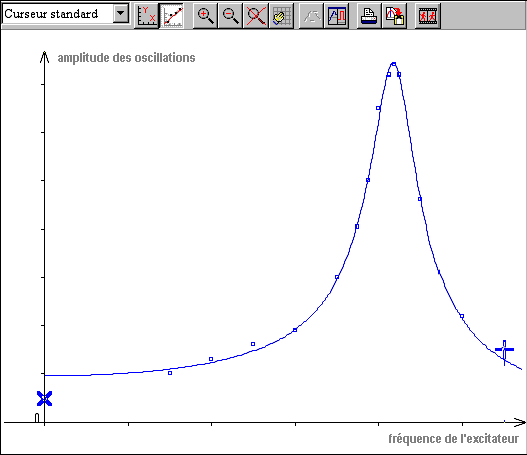
\includegraphics[width=.5 \linewidth]{resonnance.png}
    \caption{Amplitude d'un oscillateur en fonction de la fréquence d'excitation.}
    \label{resonnanceI}
\end{figure}

\begin{encadre}
    Lorsque deux oscillateurs de même fréquence sont reliés entre eux, le premier communique progressivement son énergie au deuxième, ils sont en \motcle{résonance}.
\end{encadre}

\newpage

\section{Oscillateurs couplés}
Lorsque deux pendules de même fréquence sont couplés, ils entrent en résonance et toute l'énergie du premier va être communiquée au deuxième qui la communique à son tour au premier et ainsi de suite. Ce transfert est d'autant plus efficace si leurs fréquences naturelles sont proches et que le couplage est rigide.

\begin{figure}[ht!]
    \centering
    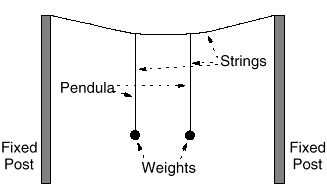
\includegraphics[width=.5 \linewidth]{resonnance_II.png}
    \caption{Deux oscillateurs de même fréquence propre rentrent en résonance lorsqu'ils sont couplés.}
    \label{resonnanceII}
\end{figure}

Si un grand nombre d'oscillateurs sont couplés de manière à former une chaîne, la perturbation du premier va progressivement se transmettre le long de cette chaîne. Il en résulte une propagation d'énergie sous forme d'énergie cinétique et potentielle sans que les oscillateurs ne se déplacent le long de la chaîne, c'est une \motcle{onde}.

\begin{figure}[ht!]
    \centering
    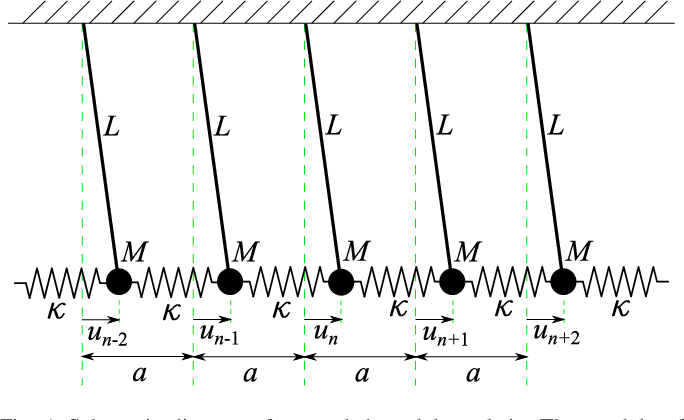
\includegraphics[width=.5 \linewidth]{resonnance_III.png}
    \caption{Cinq oscillateurs couplés.}
    \label{resonnanceIII}
\end{figure}


\begin{encadre}
    Une \motcle{onde mécanique} est un transfert de proche en proche d'un signal à travers un milieu ; ce signal consiste en la modification d'une propriété physique du milieu : position de la matière, pression, ...
    La propagation d'une onde s'accompagne d'un transfert d'énergie, mais pas d'un transfert de matière.
\end{encadre}
